\section{Robot}

\subsection{Schéma de câblage}

\begin{figure}[H]
\centering
\begin{minipage}{.5\textwidth}
  \centering
  \centerline{\includegraphics[width=1.5\linewidth]{pdf/cablages.pdf}}
  \captionof{figure}{\emph{Schéma de cablâge simplifié du robot}}
  \label{fig:schcablage}
\end{minipage}%
\end{figure}

\vfill
\noindent\makebox[\linewidth]{\rule{.8\paperwidth}{.6pt}}\\[0.2cm]
I.U.T. Nice Côte d'Azur - SAE Robot - 2023 \hfill goofyBot
\noindent\makebox[\linewidth]{\rule{.8\paperwidth}{.6pt}}
\newpage

\subsection{Électronique}

Afin que notre robot fonctionne, il faut qu'il soit alimenté, et que toute l'électronique fonctionne correctement.

Le robot reçoit en entrée sur la carte batterie une tension de 12V mais les cartes électroniques doivent être alimentées en 5V et en 3.3V pour fonctionner. 
Ainsi sur nos cartes il y a des composants actifs qui jouent des rôles importants.
Nous avons premièrement des régulateurs de tension qui sont sur la carte de commande et qui génèrent du 5V ou du 3.3V pour alimenter le microcontrôleur, et les différentes cartes électroniques.

\begin{figure}[H]
\centering
\begin{minipage}{.5\textwidth}
  \centering
  \includegraphics[width=.8\linewidth]{img/composants/tsr.png}
  \captionof{figure}{\emph{régulateur 12V à 5V}}
  \label{fig:tsr}
\end{minipage}%
\begin{minipage}{.5\textwidth}
  \centering
  \includegraphics[width=.8\linewidth]{img/composants/l78l.png}
  \captionof{figure}{\emph{régulateur 5V à 3.3V}}
  \label{fig:l78l}
\end{minipage}
\end{figure}

Dans l’autre sens, nous avons des optocoupleurs à entrée inverseurs sur la carte commande qui servent à prendre la tension de sortie du microcontrôleur et la transformer en une tension de 12V à appliquer aux bornes du moteur, en faisant passer le courant 2 fois dedans pour récupérer le même signal mais augmenté.

Nous avons un capteur de fin de course qui est connecté sur la borne + au contact normalement ouvert et la borne - au commun du capteur. Le circuit est donc fermé lorsque le fin de course est activé et ainsi le capteur envoie une valeur analogique de 1 lorsqu'il est fermé.
Il nous a fallu aussi intégrer le concept de résistance de pull-up/pull-down. Dans un montage Pull-up il y a une résistance est appelée Pull-up lorsque elle est directement connectée a l'entrée d'alimentation et que lorsque le bouton poussoir est enfoncée son entrée est 0 en état actif. Et inversement, un montage Pull-down intégre une résistance de Pull-down qui est reliée a la masse et l'entrée logique quand le bouton est activé est 1.       

\vfill
\noindent\makebox[\linewidth]{\rule{.8\paperwidth}{.6pt}}\\[0.2cm]
I.U.T. Nice Côte d'Azur - SAE Robot - 2023 \hfill goofyBot
\noindent\makebox[\linewidth]{\rule{.8\paperwidth}{.6pt}}
\newpage

\begin{figure}[H]
\centering
\begin{minipage}{.5\textwidth}
  \centering
  \centerline{\includegraphics[width=1\linewidth]{img/cartes/tor.jpeg}}
  \captionof{figure}{\emph{capteur TOR Fin de Course}}
  \label{fig:tor}
\end{minipage}%
\end{figure}

\begin{figure}[H]
\centering
\begin{minipage}{.5\textwidth}
  \centering
  \includegraphics[width=.8\linewidth]{img/cartes/moteur.jpeg}
  \captionof{figure}{\emph{Roue + Moteur}}
  \label{fig:moteur}
\end{minipage}%
\begin{minipage}{.5\textwidth}
  \centering
  \includegraphics[width=.8\linewidth]{img/cartes/moteurs.jpeg}
  \captionof{figure}{\emph{Essieu}}
  \label{fig:essieu}
\end{minipage}
\end{figure}

\subsection{Cartes}
Pour mener à bien notre projet nous avons eu besoin de concevoir 3 cartes électroniques : la carte IHM, la carte capteurs et la carte hacheur. Pour cela nous avons dû utiliser le logiciel DesignSpark PCB, qui est un logiciel de conception de circuits imprimés (PCB) gratuit développé par RS Components, une entreprise de distribution de composants électroniques. 

\vfill
\noindent\makebox[\linewidth]{\rule{.8\paperwidth}{.6pt}}\\[0.2cm]
I.U.T. Nice Côte d'Azur - SAE Robot - 2023 \hfill goofyBot
\noindent\makebox[\linewidth]{\rule{.8\paperwidth}{.6pt}}
\newpage


Il permet aux utilisateurs de concevoir des schémas électriques, de créer des circuits imprimés et de générer des fichiers de fabrication pour la production de PCB.

\begin{figure}[H]
\centering
\begin{minipage}{.5\textwidth}
  \centering
  \centerline{\includegraphics[width=1.5\linewidth]{img/dspcb.png}}
  \captionof{figure}{\emph{Interface utilisateur de DesignSpark PCB}}
  \label{fig:dspcb}
\end{minipage}%
\end{figure}

\subsubsection{Carte Batterie}

La carte batterie pour le projet est utilisée pour alimenter les différents composants du robot, tels que les moteurs, les capteurs et le microcontrôleur. 
L’objectif de cette carte est de contrôler la tension d’entrée d’alimentation du robot pour assurer un bon fonctionnement nominal et assurer que celui-ci ne s'arrête pas en pleine course.

Cette carte est composée premièrement par un comparateur de tension qui se base pour sa comparaison sur la tension d’une diode zener, réputée pour sa stabilité, et grâce à un pont diviseur,cette tension est comparée avec la tension d’entrée pour s'assurer que la batterie est chargée et délivre une tension de 12V. 
Une led de mise sous tension s’allume et si la tension est supérieure à 12V une led verte s’allume et si cette tension est inférieure à 12V elle ne s’allume pas.


Cette carte est composée aussi d’un shunt qui permet de vérifier que la comparaison est faite en mettant une tension de comparaison volontairement inférieure à 12V et un fusible qui protège les composants.
Sur le haut, il y a des connecteurs qui permettent d’alimenter les cartes commande et hacheur et un interrupteur qui permet de gérer l’alimentation du robot.

\vfill
\noindent\makebox[\linewidth]{\rule{.8\paperwidth}{.6pt}}\\[0.2cm]
I.U.T. Nice Côte d'Azur - SAE Robot - 2023 \hfill goofyBot
\noindent\makebox[\linewidth]{\rule{.8\paperwidth}{.6pt}}
\newpage

\begin{figure}[H]
\centering
\begin{minipage}{.3\textwidth}
  \centering
  \centerline{\includegraphics[width=1\linewidth, angle = -90]{img/cartes/batterie.jpeg}}
  \captionof{figure}{\emph{Carte Batterie}}
  \label{fig:batterie}
\end{minipage}%
\end{figure}

\vfill
\noindent\makebox[\linewidth]{\rule{.8\paperwidth}{.6pt}}\\[0.2cm]
I.U.T. Nice Côte d'Azur - SAE Robot - 2023 \hfill goofyBot
\noindent\makebox[\linewidth]{\rule{.8\paperwidth}{.6pt}}
\newpage


\subsubsection{Carte IHM}

La carte IHM (Interface Homme-Machine) est un élément clé de notre projet. Elle a pour rôle de 
permettre à l'utilisateur de contrôler et de visualiser l'état du système de manière intuitive.
La carte IHM est principalement constituée de boutons poussoirs et de LEDs. Elle est connectée au microcontrôleur via une interface de communication (la carte commande), qui lui permet de recevoir des informations et de transmettre des commandes.

Les boutons poussoirs sont des interrupteurs à bascule qui sont actionnés par une pression sur leur surface. Ils peuvent être utilisés pour lancer une action ou basculer entre différents états. 

Dans le cas de la SAE, ils seront utilisés pour sélectionner le programme ou choisir des valeurs.
Les LEDs sont des composants électroniques qui émettent de la lumière lorsqu'ils sont alimentés par du courant électrique. Elles peuvent être utilisées pour indiquer l'état d'un système, en affichant une couleur différente en fonction de l'état.

\begin{figure}[H]
\centering
\begin{minipage}{.5\textwidth}
  \centering
  \centerline{\includegraphics[width=1\linewidth]{img/cartes/ihm.jpeg}}
  \captionof{figure}{\emph{carte IHM}}
  \label{fig:ihm}
\end{minipage}%
\end{figure}

\vfill
\noindent\makebox[\linewidth]{\rule{.8\paperwidth}{.6pt}}\\[0.2cm]
I.U.T. Nice Côte d'Azur - SAE Robot - 2023 \hfill goofyBot
\noindent\makebox[\linewidth]{\rule{.8\paperwidth}{.6pt}}
\newpage

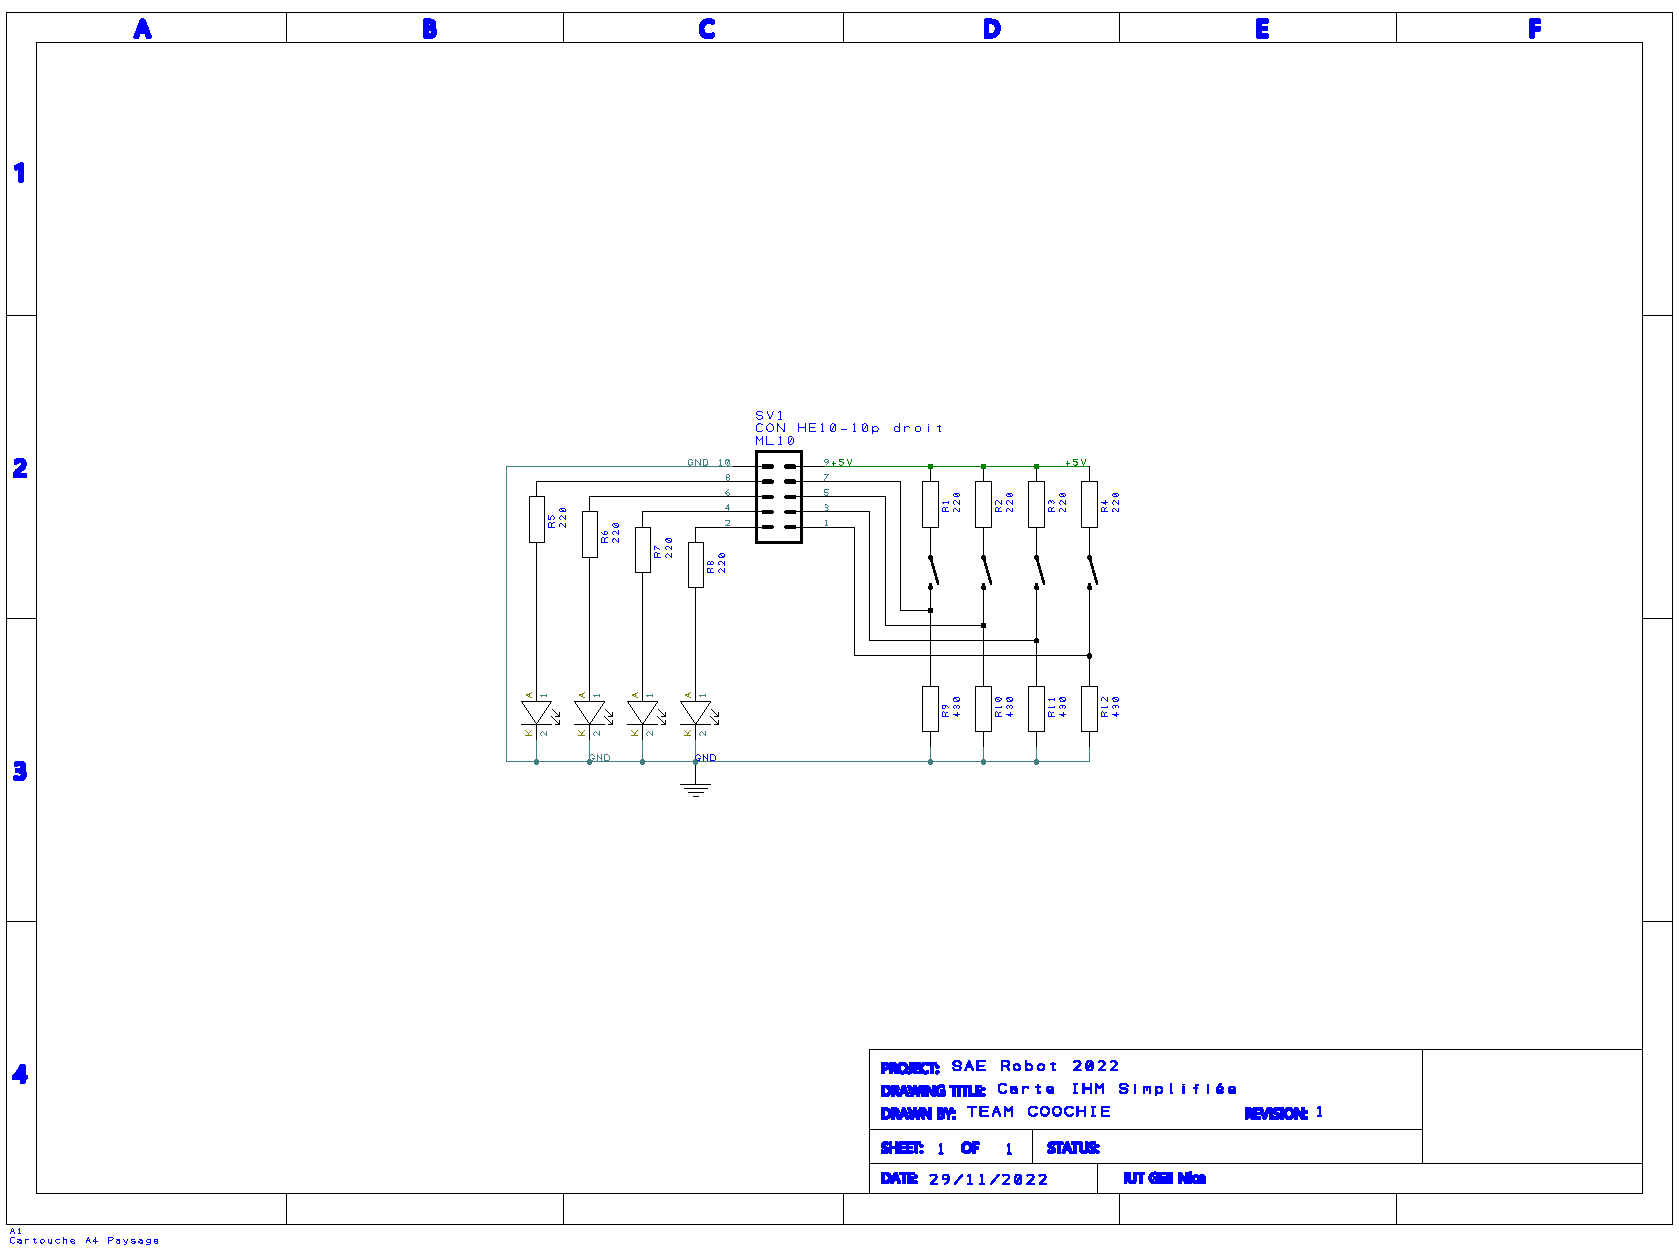
\includepdf[pages=-]{pdf/cartes/ihm/IHM - Project.pdf}
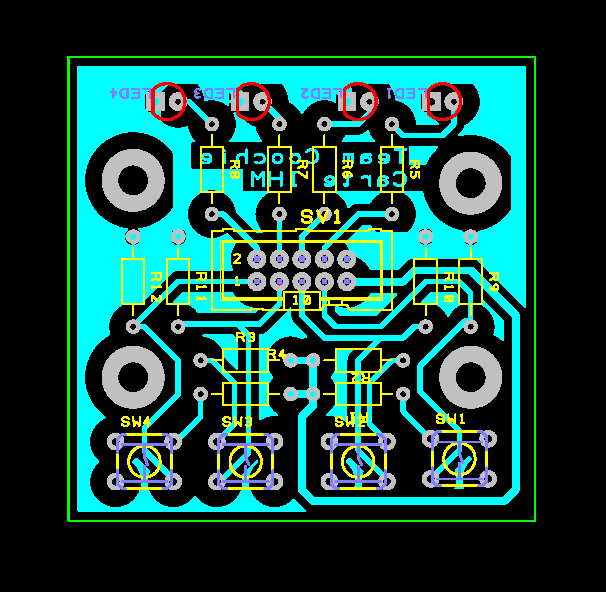
\includepdf[pages=-]{pdf/cartes/ihm/IHM - PCB.pdf}

\subsubsection{Carte Capteurs}

La carte capteur est une carte qui a pour objectif de détecter la ligne blanche pour diriger le robot.
Elle est composée de 4 capteurs TCRT5000L faits de phototransistors qui ont la particularité de laisser passer le courant quand son signal infrarouge envoyé est capté, c’est a dire lorsque il est au-dessus d’une surface blanche.

\begin{figure}[H]
\centering
\begin{minipage}{.5\textwidth}
  \centering
  \centerline{\includegraphics[width=0.6\linewidth]{img/composants/tcrt5000.png}}
  \captionof{figure}{\emph{Capteur TCRT5000}}
  \label{fig:tcrt5000}
\end{minipage}%
\end{figure}
Nous avons choisi ces derniers pour leur épaisseur plutôt négligeable et car nous avions réalisé des études préliminaires dessus et avons conclu que la différence de potentiel entre une surface blanche ou noire était la plus significative.

Parmi les quatre capteurs, deux sont en permanence sur la ligne a 19 mm de distance pour s'assurer de rester centré sur la ligne et se re-guider sur la ligne dans le cas où un des deux capteurs détectent une déviation de trajectoire jusqu'à ce que la ligne soit retrouvée.


Les deux autres sont aux plus aux extrémités du robot, comme des capteurs d’urgence pour plusieurs raisons : identifier un espacement pour comprendre que le robot traverse les confettis, pour détecter la ligne dans le cas ou le robot perdrait le signal des deux capteurs centraux, pour encore une fois se redresser et de nouveau recevoir un signal de ligne blanche au centre et aussi pour identifier les raccourcis disponibles sur le circuit quand l’un d’eux est aperçu.


Ainsi dans l’épreuve des confettis tant que les quatre capteurs n’ont pas détecté une zone blanche le robot va tout droit et dans l’épreuve du suivi de ligne, nous suivons une machine à état précise qui nous permet d’aller jusqu'à la fin du parcours avec les capteurs servant donc à garder le robot sur la ligne.


Sur le PCB nous voyons les capteurs branchés chacun à deux résistances en série pour fixer le courant qui circule et le transformer en une tension mesurable.
Notre carte capteurs est désignée particulièrement dans notre équipe car nous avons choisi ce design pensant que le capteur serait plus performant pour re-capter la ligne dans les cas extrêmes.

\vfill
\noindent\makebox[\linewidth]{\rule{.8\paperwidth}{.6pt}}\\[0.2cm]
I.U.T. Nice Côte d'Azur - SAE Robot - 2023 \hfill goofyBot
\noindent\makebox[\linewidth]{\rule{.8\paperwidth}{.6pt}}
\newpage

Les capteurs sont reliés à la carte de commande qui enverra les données des capteurs au microcontrôleur qui traitera les informations pour agir sur le mouvement du robot par le biais de la carte hacheur.

\begin{figure}[H]
\centering
\begin{minipage}{.5\textwidth}
  \centering
  \centerline{\includegraphics[width=1.5\linewidth]{img/cartes/capteur.jpeg}}
  \captionof{figure}{\emph{Carte 4 capteurs}}
  \label{fig:cartecapteurs}
\end{minipage}%
\end{figure}

\vfill
\noindent\makebox[\linewidth]{\rule{.8\paperwidth}{.6pt}}\\[0.2cm]
I.U.T. Nice Côte d'Azur - SAE Robot - 2023 \hfill goofyBot
\noindent\makebox[\linewidth]{\rule{.8\paperwidth}{.6pt}}
\newpage

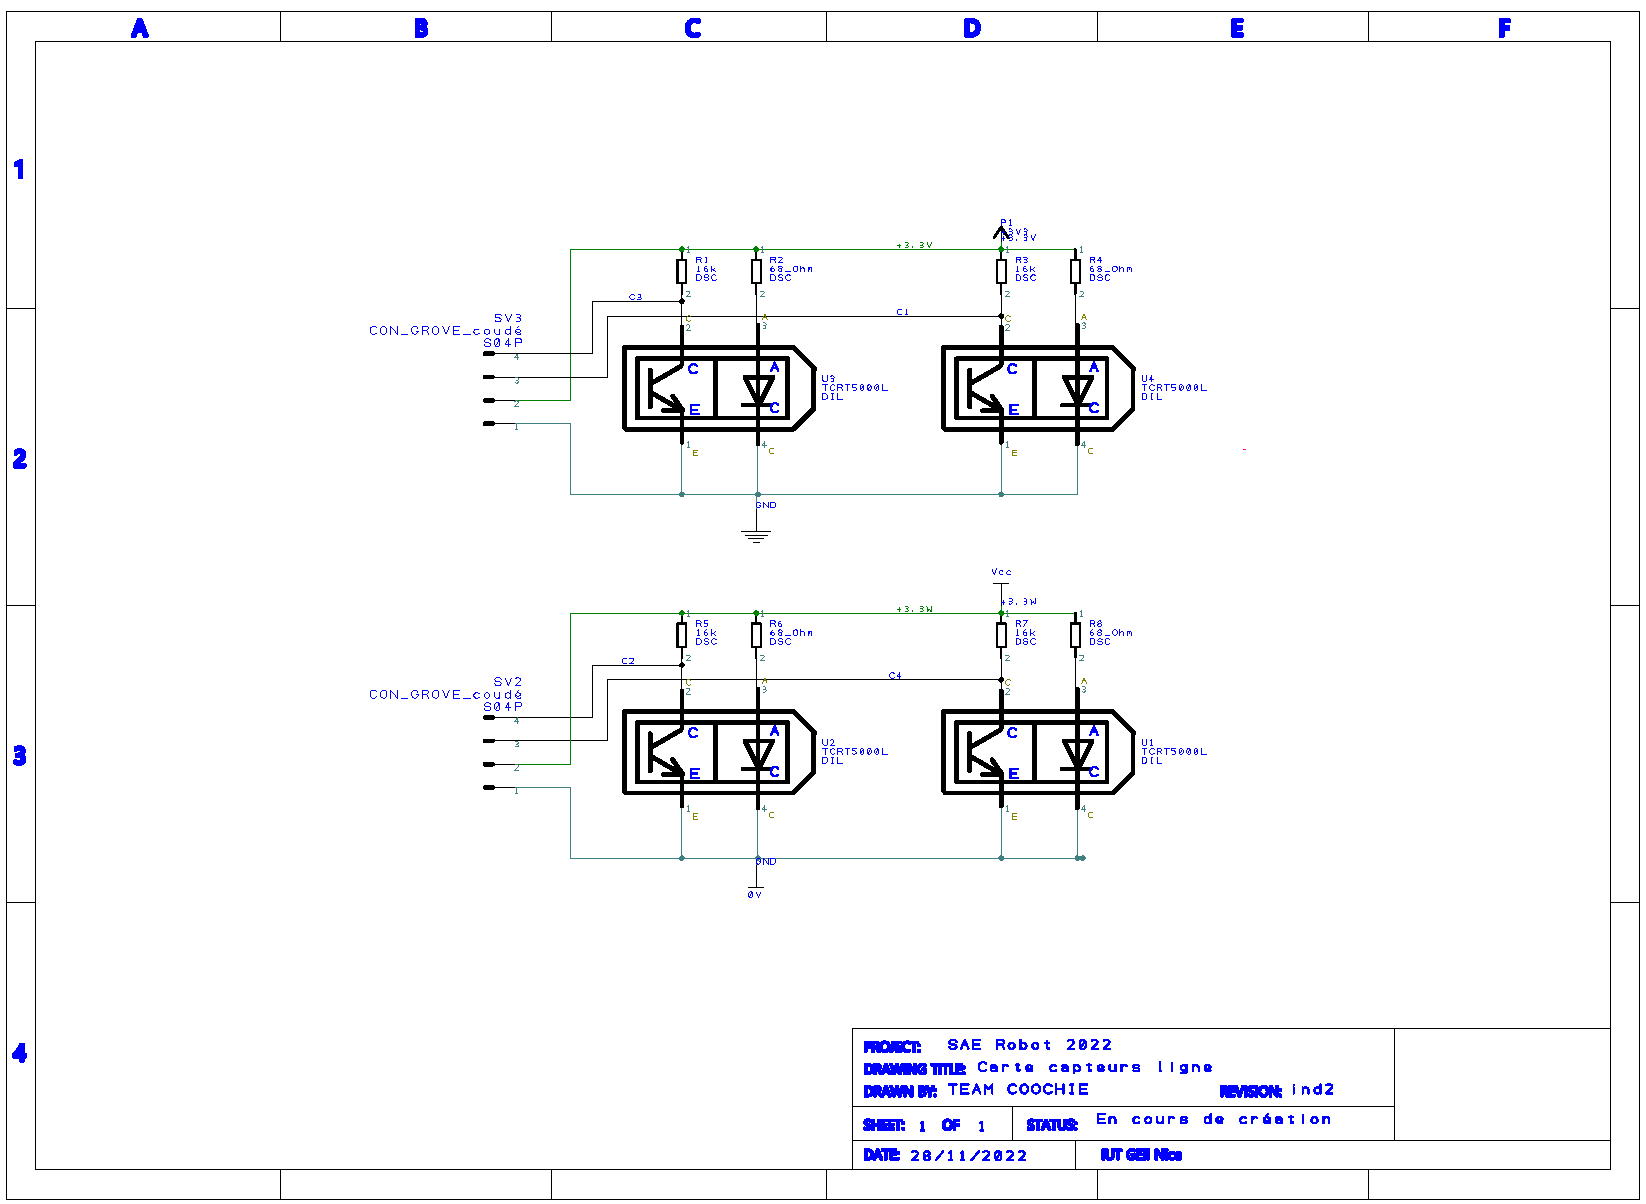
\includepdf[pages=-]{pdf/cartes/capteurs/CartesCapteurs - Project.pdf}

\includepdf[pages=-]{pdf/cartes/capteurs/CartesCapteurs - PCB.pdf}

\subsubsection{Carte Hacheur}
La carte hacheur est une carte qui doit gérer la vitesse des moteurs dans l’optique de contrôler les déplacements du robot car pour répondre au cahier des charges nous devons pouvoir faire varier la vitesse des moteurs et leur sens.


L’objectif de la carte est d’obtenir une tension de sortie variable pour nous permettre le contrôle des moteurs dans les 4 quadrants afin de pouvoir accélérer et freiner dans les 2 sens qui sont avant et arrière.


Nous avons trouvé en séance de projet tuteuré la solution pour contrôler les moteurs et c’est le composant L298 qui sera intégré à notre carte.
Il est constitué de 2 ponts-H avec chacun 2 transistors servant à amplifier la tension pour délivrer du 12V aux bornes de 2 moteurs et aussi à changer le sens de rotation des moteurs en inversant le sens de courant qui les traverse.
On peut ainsi faire varier la vitesse des moteurs avec le micro-contrôleur en faisant varier l’entrée logique rapport cyclique de chacun et ainsi faire rouler le robot à la vitesse souhaitée ou le faire tourner.
Avec ses entrées de sens et de PWM pour chaque moteur, il prend donc place au milieu de notre carte électronique de contrôle intégral des moteurs du robot.


Nous voyons donc qu’en plus du composant nous avons des diodes de roue libre pour protéger les transistors et des condensateurs utilisés comme filtres passifs qui servent à lisser la tension d’entrée et la stabiliser.


\begin{figure}[H]
\centering
\begin{minipage}{.5\textwidth}
  \centering
  \includegraphics[width=.6\linewidth, angle = -90]{img/cartes/hacheur.jpeg}
  \captionof{figure}{\emph{Carte Hacheur}}
  \label{fig:hacheur}
\end{minipage}
\end{figure}

\vfill
\noindent\makebox[\linewidth]{\rule{.8\paperwidth}{.6pt}}\\[0.2cm]
I.U.T. Nice Côte d'Azur - SAE Robot - 2023 \hfill goofyBot
\noindent\makebox[\linewidth]{\rule{.8\paperwidth}{.6pt}}
\newpage

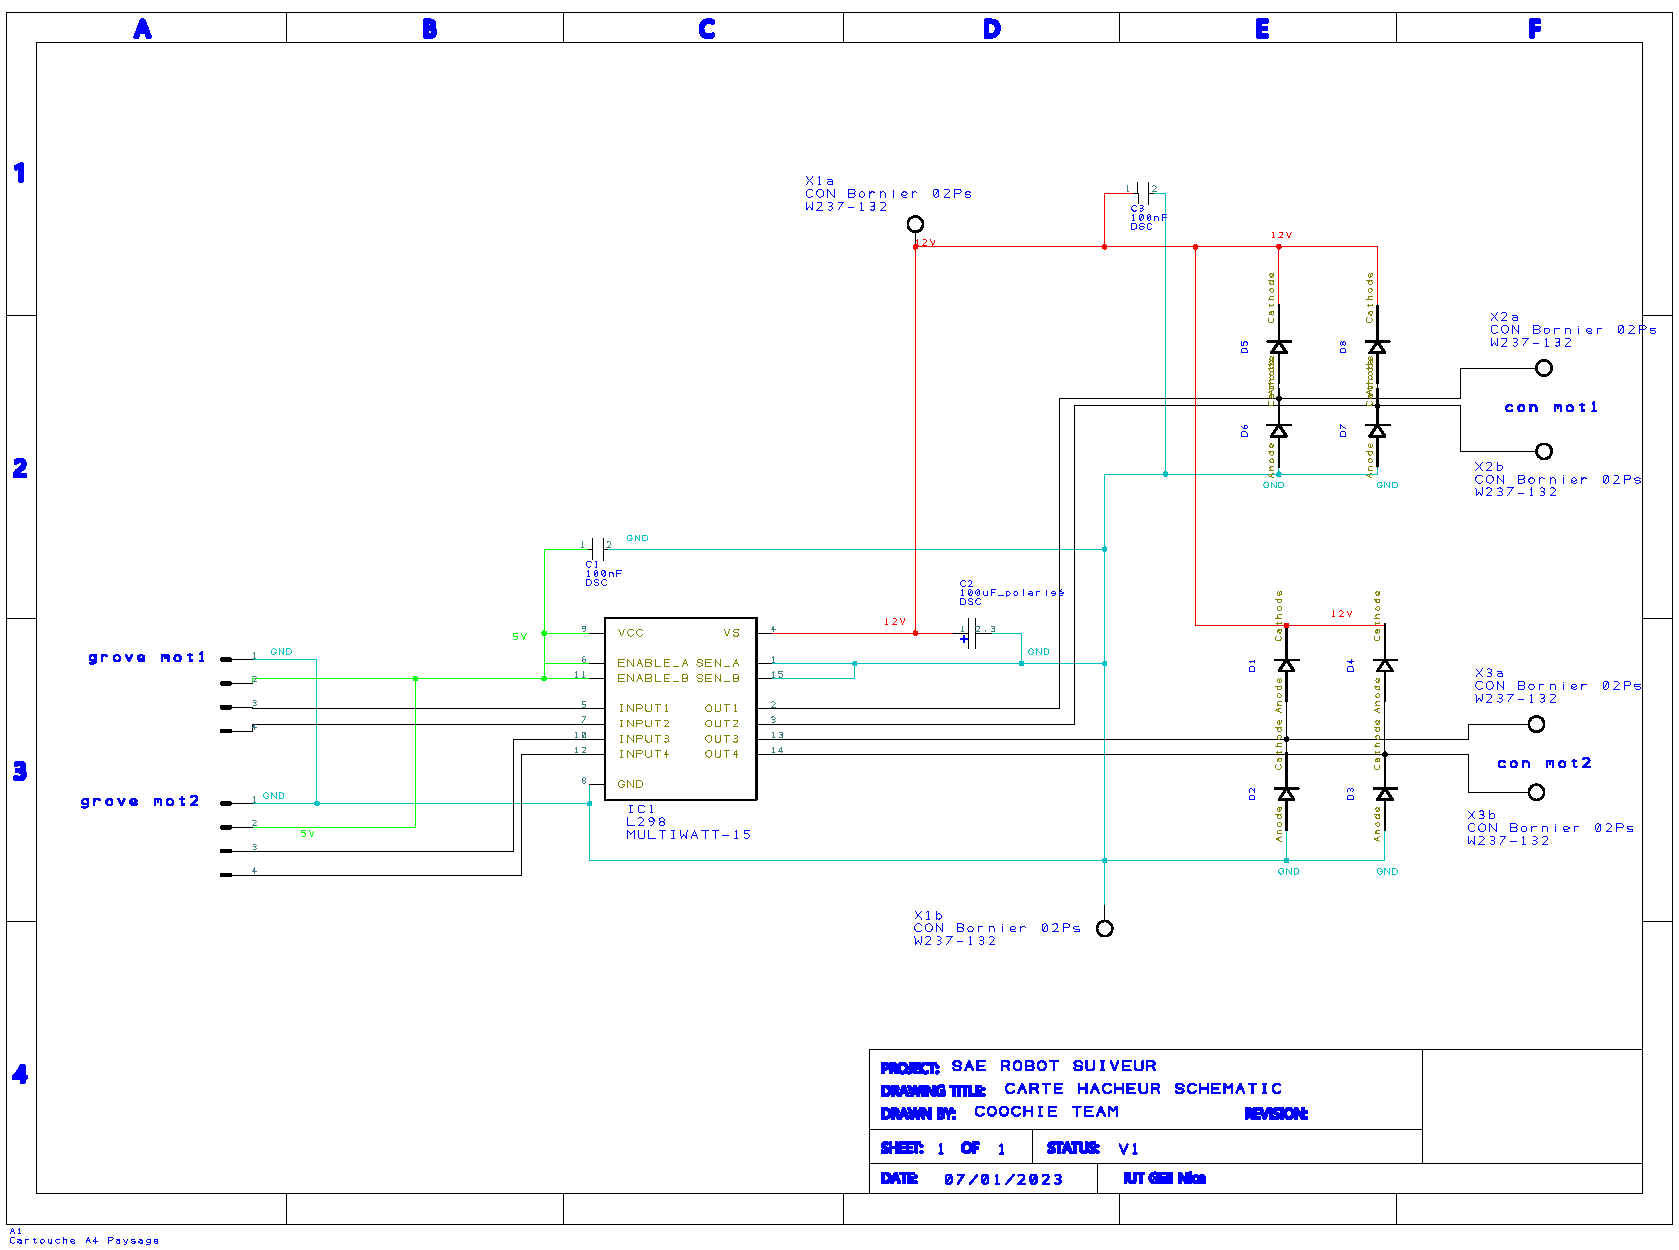
\includepdf[pages=-]{pdf/cartes/hacheur/CarteHacheur - Project.pdf}

\includepdf[pages=-]{pdf/cartes/hacheur/CarteHacheur - PCB.pdf}

\subsubsection{Carte Commande}

La carte commande est un composant électronique qui permet de contrôler les mouvements du robot. Elle utilise les entrées provenant des capteurs de suivi de ligne pour déterminer où se trouve le robot par rapport à la ligne et donne les instructions nécessaires pour que le robot la suive.

L'utilité de cette carte de commande est d'adapter le système global au format de la MBED. Elle permet de réguler la tension selon en fonction des composants du robot (5V pour la Mbed, 3.3V pour les capteurs etc.). elle permet aussi d'avoir une carte où les entrées et sorties sont centralisées (bornier Grove, octocoupleurs, etc.).
La carte est connectée aux pins GPIO du micro-contrôleur, et rassemble ainsi les informations provenant des capteurs et distribue les ordres du microcontrôleur selon le programme sélectionné.


\begin{figure}[H]
\centering
\begin{minipage}{.5\textwidth}
  \centering
  \centerline{\includegraphics[width=1\linewidth, angle = 90]{img/cartes/commande.jpeg}}
  \captionof{figure}{\emph{Carte Commande}}
  \label{fig:cmd}
\end{minipage}%
\end{figure}

\subsection{Micro-contrôleur}

Le micro-contrôleur est le cerveau de ce projet. En effet, c'est un circuit intégré qui rassemble les éléments essentiels d'un ordinateur : processeur, mémoires (mémoire morte et mémoire vive), unités périphériques et interfaces d'entrées-sorties. 

\vfill
\noindent\makebox[\linewidth]{\rule{.8\paperwidth}{.6pt}}\\[0.2cm]
I.U.T. Nice Côte d'Azur - SAE Robot - 2023 \hfill goofyBot
\noindent\makebox[\linewidth]{\rule{.8\paperwidth}{.6pt}}
\newpage

Dans notre projet, nous utilisons la plateforme de développement FRDM-KL25Z imposée, conçue par l'entreprise Freescale Semiconductor Inc., filiale de NXP. Elle est équipée d'un micro-contrôleur Arm Cortex-M0+ de 48 MHz, 128 KB de mémoire flash (ROM), 16 KB de mémoire vive (RAM). De plus, la MBED est équipée de plusieurs pins GPIO d'entrée/sortie numériques, d'entrée analogiques et de sortie PWM permettant de reçevoir des données et d'interagir avec les moteurs du robot.

En utilisant le logiciel de développement intégré (IDE) Keil Arm Studio Cloud, nous avons pu développer notre code du contrôle du robot en langage C++ (cf. Programmation). À la compilation, l'IDE Keil Studio fournit un fichier \emph{.bin} qui est à placer à la racine du système de fichiers de la MBED. 

\begin{figure}[H]
\centering
\begin{minipage}{.5\textwidth}
  \centering
  \centerline{\includegraphics[width=1\linewidth]{img/composants/frdmkl25z.png}}
  \captionof{figure}{\emph{Plateforme de développement FRDM KL25Z}}
  \label{fig:frdmkl25z}
\end{minipage}%
\end{figure}

\vfill
\noindent\makebox[\linewidth]{\rule{.8\paperwidth}{.6pt}}\\[0.2cm]
I.U.T. Nice Côte d'Azur - SAE Robot - 2023 \hfill goofyBot
\noindent\makebox[\linewidth]{\rule{.8\paperwidth}{.6pt}}
\newpage